\documentclass[a4paper,12pt]{article} 

%%% Работа с русским языком
\usepackage{cmap}                           % поиск в PDF
\usepackage{mathtext} 			 	       % русские буквы в формулах
\usepackage[T2A]{fontenc}               % кодировка
\usepackage[utf8]{inputenc}              % кодировка исходного текста
\usepackage[english,russian]{babel}  % локализация и переносы
\usepackage[left=2cm,right=2cm,
    top=2cm,bottom=3cm,bindingoffset=0cm]{geometry}
\usepackage{wrapfig}
\usepackage{gensymb}
\usepackage{textcomp}
\usepackage{multirow}
\usepackage{amsmath,amsfonts,amssymb,amsthm,mathtools} % AMS
\usepackage{euscript}	 % Шрифт Евклид
\usepackage{mathrsfs} % Красивый матшрифт
\usepackage{graphicx}%Вставка картинок правильная
\usepackage{float}%"Плавающие" картинки
\usepackage{wrapfig}%Обтекание фигур (таблиц, картинок и прочего)
\title{Лабораторная работа 3.3.6 

Влияние магнитного поля на проводимость полупроводников}
\author{Кагарманов Радмир Б01-106}
\date{7 ноября 2022 г.}

\begin{document}
\maketitle
\thispagestyle{empty}
\newpage
\setcounter{page}{1}

\paragraph{Цель работы:} исследовать зависимость напряжения на образце от величины магнитного поля и от ориентации образца в магнитном поле.

\paragraph{В работе используется:} стабилизированный источник постоянного тока и напряжения, электромагнит, цифровой вольтметр, амперметр, миллиамперметр, реостат, измеритель магнитной индукции, образцы - монокристаллического антимонида индия n-го типа.

\paragraph{Экпериментальная установка\\}
Схема установки для исследования магнетосопротивления полупроводников и геометрического резистивного эффекта представлена на рис. 1.\par
\begin{figure}[!h]
\centering
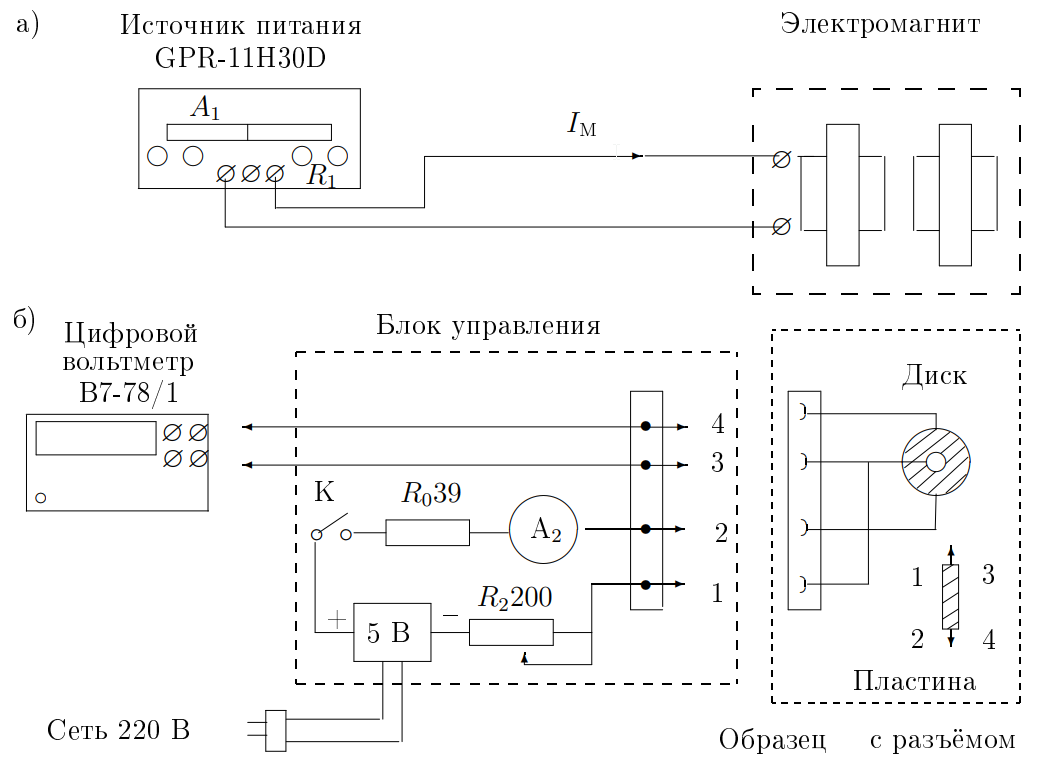
\includegraphics[width=0.9\linewidth]{установка.png}
\caption{Экспериментальная установка}
\label{fig:mpr}
\end{figure}
В зазоре электромагнита (рис. 1а) создаётся постоянное магнитное поле, величину которого можно менять с помощью источника питания электромагнита. Ток электромагнита измеряется амперметром $A_1$. Магнитная индукция в зазоре измеряется при помощи милливеберметра или миллитесламетра на основе датчика Холла. \par
Образец в форме кольца (диск Корбино) или пластинки, смонтированный в специальном держателе, подключается к источнику постоянного напряжения 5 В. При замыкании ключа $K_2$ сквозь образец течёт ток, величина которого измеряется миллиамперметром $A_2$ и регулирется реостатом $R_2$. Балластное сопротивление $R_0$ ограничивает ток через образец. Измеряемое напряжение подаётся на вход вольтметра $V$. 
\newpage

\paragraph{Обработка результатов\\}
\subparagraph{1.} Построим график $B=f(I_{м})$.
\begin{figure}[!h]
\centering
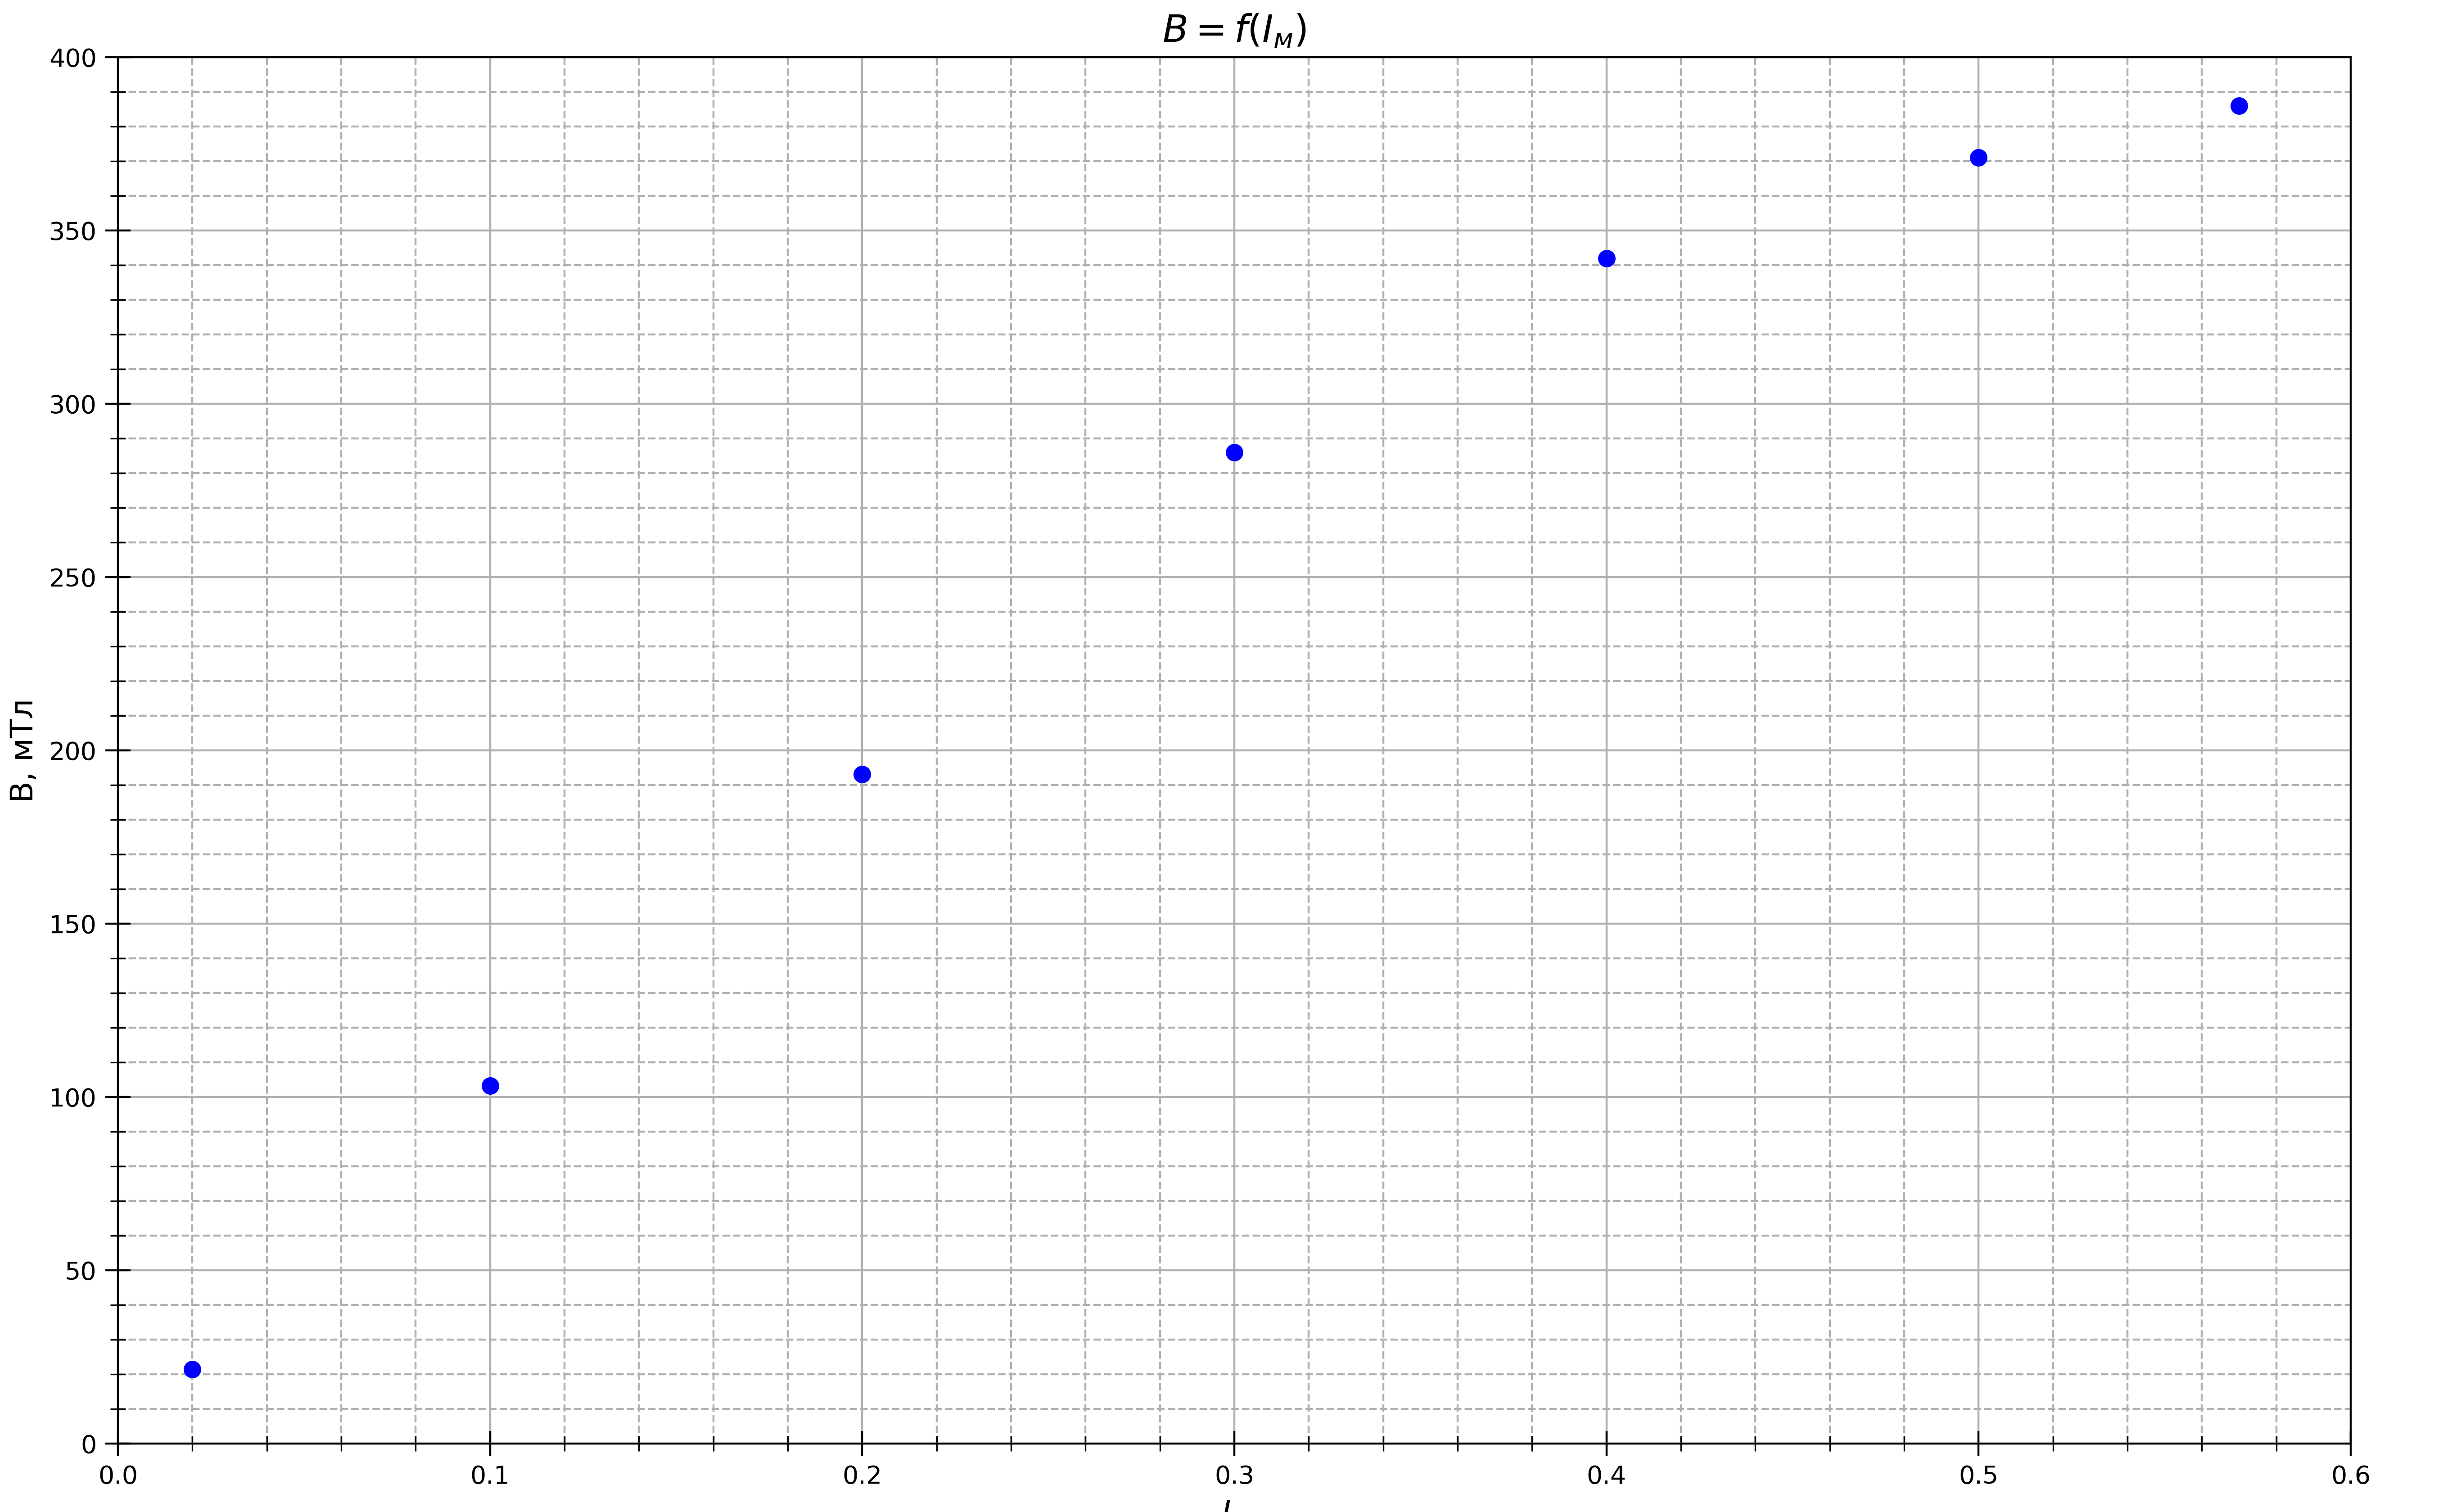
\includegraphics[width=0.9\linewidth]{graph1.png}
\caption{$B=f(I_{м})$}
\label{fig:mpr}
\end{figure}

\subparagraph{2.}На рис. 2 изображены графики $R=f(I_{м})$ для диска Корбино и пластины.
\begin{figure}[!h]
\centering
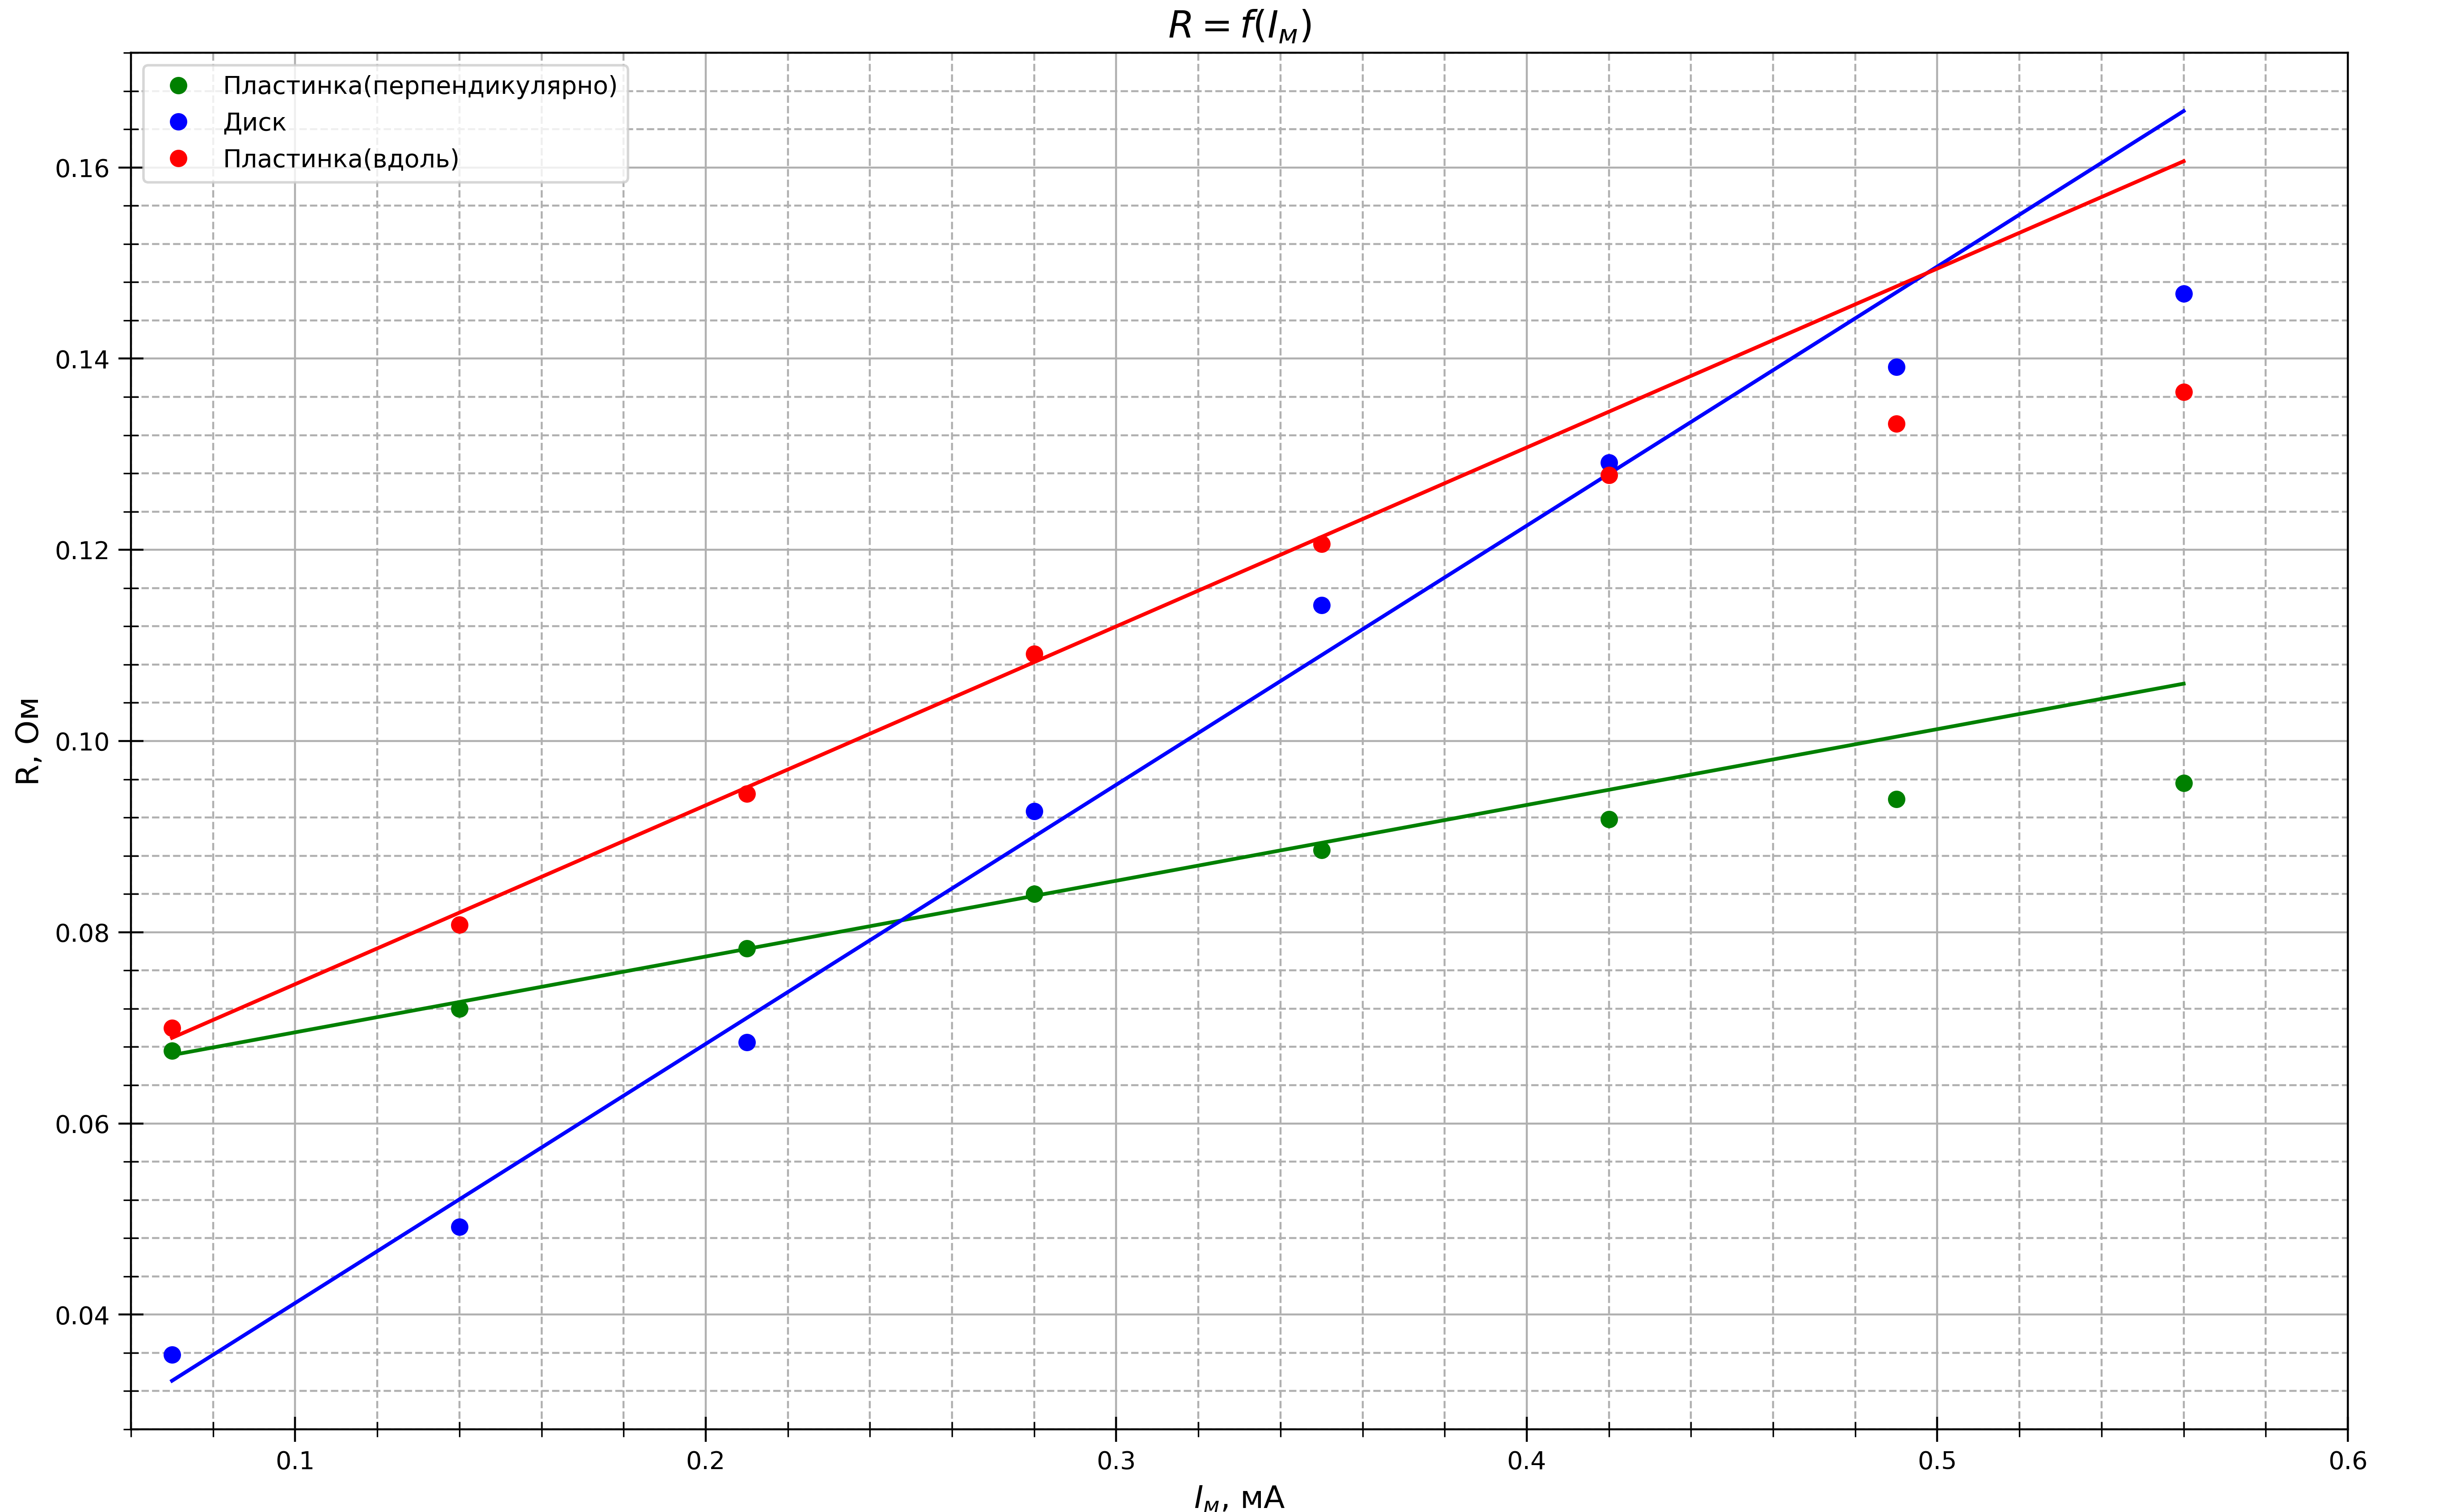
\includegraphics[width=0.9\linewidth]{graph2.png}
\caption{$B=f(I_{м})$}
\label{fig:mpr}
\end{figure}
\newpage
\subparagraph{3.}Зная сопротивление образца в отсутствии магнитного поля, можно рассчитать удельное сопротивление образца по формуле $R_0 = \frac{\rho_0}{2\pi r h}ln\frac{r2}{r1}$.
\begin{center}
    $\rho_0 = 2,9 \cdot 10^{-7}~ Ом\cdot м$
\end{center}
\paragraph{Вывод:} в данной работе мы исследовали заваисимость напряжения на образце от величины магнитного поля и от ориентации образца в магнитном поле, вычислили $\rho_0 = 2,9 \cdot 10^{-7}~ Ом\cdot м$.
\end{document}
